\documentclass[a4paper,10pt]{article}

\usepackage{url}

\usepackage[T1]{fontenc}
\usepackage[utf8]{inputenc}
\usepackage[spanish, es-tabla]{babel}

\clubpenalty=10000
\widowpenalty=10000

\usepackage[gen]{eurosym}

\usepackage{xcolor}
\usepackage{setspace}
\usepackage{float}
\usepackage{biblatex}
\addbibresource{fuentes.bib}
\setlength{\parindent}{0cm}
\usepackage{amsmath, amssymb}
\usepackage{svg}
\usepackage{multirow}

% Listados de código
\usepackage{minted}
\usepackage{caption}
\newenvironment{code}{\captionsetup{type=listing}}{}
% \SetupFloatingEnvironment{listing}{name=Source Code}
\renewcommand{\listingscaption}{Código}
\BeforeBeginEnvironment{minted}{\vspace{-.3cm}}
\AfterEndEnvironment{minted}{\vspace{-.3cm}}

\usepackage{csquotes}

\renewcommand{\it}[1]{\textit{#1}}
\renewcommand{\bf}[1]{\textbf{#1}}
\renewcommand{\tt}[1]{\texttt{#1}}

% Define el comando para introducir código
 \newenvironment{codigo}[1]
 {
    \captionsetup{type=listing}
    \VerbatimEnvironment
    \begin{minted}[fontsize=\normalsize, xleftmargin=0pt, xrightmargin=0pt, frame=lines]{#1}}
 {\end{minted}}

\usepackage{booktabs} % Allows the use of \toprule, \midrule and \bottomrule in tables for horizontal lines
\usepackage{graphicx}
\graphicspath{{imagenes/}{../imagenes/}} % Declara dos paths, uno con respecto a este documento y otro respecto a la carpeta secciones

\parskip=0.4cm % Distancia entre párrafos

\usepackage[margin=3cm, headheight=18.9627pt]{geometry}
 \usepackage{fancyhdr}
\fancyhf{}
\lhead{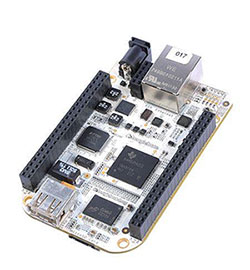
\includegraphics[width=0.5cm]{product_beaglebone.jpg}}
\fancyhead[C]{\emph{Sistemas Empotrados 2 -- 2020-21}}
\rhead{\emph{Trabajo de asignatura}}
\fancyfoot[C]{\thepage}

\usepackage{subfiles} % Permite incluir ficheros .tex en el texto

\usepackage{hyperref} % Hace que el índice sean hiperenlaces al documento


\begin{document}

\begin{titlepage}
    \centering
    
\includegraphics[width=1 cm]{logoUZ.jpg}
    
    \textsc{\large Universidad de Zaragoza}
    \rule{\textwidth}{1.6pt}\vspace*{-\baselineskip}\vspace*{2pt} % Thick horizontal rule
    \rule{\textwidth}{0.4pt} % Thin horizontal rule
    
    \vfill
    
    {\LARGE \scshape Sistemas Empotrados 2}
                
    \vspace{2cm}            

    {\bfseries \Huge Trabajo de asignatura}
    
    \vspace{.5cm} 
    
    {\bfseries \Large Medida de latencias en Linux usando Ftrace}
    
    \vspace{3cm}    
    
   

    {\scshape Autor:}


    \vspace{0.2cm}
    
    \large
    \begin{tabular}{c l l}
    \large             & Adrián Martín Marcos       & 756524 \\
     \end{tabular}

    \vfill
    
    \large{Zaragoza, España}
    
    {Curso 2020\,--\,2021}

    \vfill

    
\includegraphics[width=5.0cm]{EINA.png}
   
\end{titlepage}

\pagenumbering{Roman}


\vspace*{2cm}
\section*{\hfil Resumen \hfil}
\addcontentsline{toc}{section}{Resumen}

Este trabajo ha consistido en modificar la distribución Linux de la práctica 3, configurando el kernel y añadiendo las herramientas necesarias para medir la latencia de ciertos eventos usando la herramienta Ftrace, y con ello poder hacer una comparativa del rendimiento del sistema sobre la BeagleBone cuando se le somete a diferentes niveles de carga de trabajo.

En este documento se detallan los pasos seguidos y el análisis de los resultados obtenidos en las pruebas realizadas. Los script utilizados y otros ficheros relevantes se incluyen en un directorio llamado \it{ficheros}. 

A lo largo de la memoria se usa terminología y se dan explicaciones que pueden no ser del todo precisas o rigurosas. Algunos de los conceptos que se tratan requieren de un análisis mucho más profundo, que no ha sido posible realizar por los plazos en los que se ha realizado este trabajo. No obstante, y aunque sea de una manera más informal, se han tratado de plasmar los conceptos más importantes que se han aprendido, si bien el documentar todas las horas invertidas en investigación sobre los temas tratados sería imposible.

\pagebreak

\begin{spacing}{0.1}
\tableofcontents
\end{spacing}
%\listoffigures
%\listoftables

\pagebreak

\setcounter{page}{1}
\pagenumbering{arabic}

\pagestyle{fancy}

\subfile{secciones/1-ftrace}

\clearpage{}
\newpage

\subfile{secciones/2-kernel}

\clearpage{}
\newpage

\subfile{secciones/3-herramientas}

\clearpage{}
\newpage

\subfile{secciones/4-distribucion}

\clearpage{}
\newpage

\subfile{secciones/5-disenno-pruebas}

\clearpage{}
\newpage

\subfile{secciones/6-resultados}

\clearpage{}
\newpage

\subfile{secciones/7-conclusiones}

\clearpage{}
\newpage

\nocite{*}
\addcontentsline{toc}{section}{Referencias} % Añade en índice
\printbibliography

\end{document}

